\section{Description of the setup}\label{sec:setupdescription}

In the last chapter we saw that the \gls{shg} intensity in a given crystal is related to the point group, order parameter, band structure, etc. of that crystal via the susceptibility tensor $\chi_{ijk}$.
It is also obvious from \cref{sec:neumann} that the ideal scenario is to be able to measure as many of the numbers $\chi_{ijk}$ as possible; after all, if you only measured the $xx$ component of \cref{eq:c2eps,eq:d3deps}, you would have obtained essentially no information about your crystal whatsoever.
The \gls{shg} setup that we built (whose design is mostly credited to Torchinsky and Hsieh\citep{torchinsky_low_2014}, with some improvements by us which I will discuss below) was designed with exactly this goal in mind.
There are two key insights which make this design work: one, the light is obliquely incident on the sample so there is some component of $\bm{E}^\mathrm{in}$ directed along the sample normal, and two, we rotate the plane of incidence so that the in-plane field direction sweeps an entire $360^\circ$.
The first point allows us to measure elements of $\chi_{ijk}$ with $z$ indices\footnote{Here and unless otherwise noted I define the sample normal to be the $z$ axis.}, and the second point makes sure we get all of the $x$ and $y$ elements of $\chi_{ijk}$ too.
All of the tensor elements are thus given a chance to contribute to the \gls{shg} intensity in a given experiment.

\begin{figure}
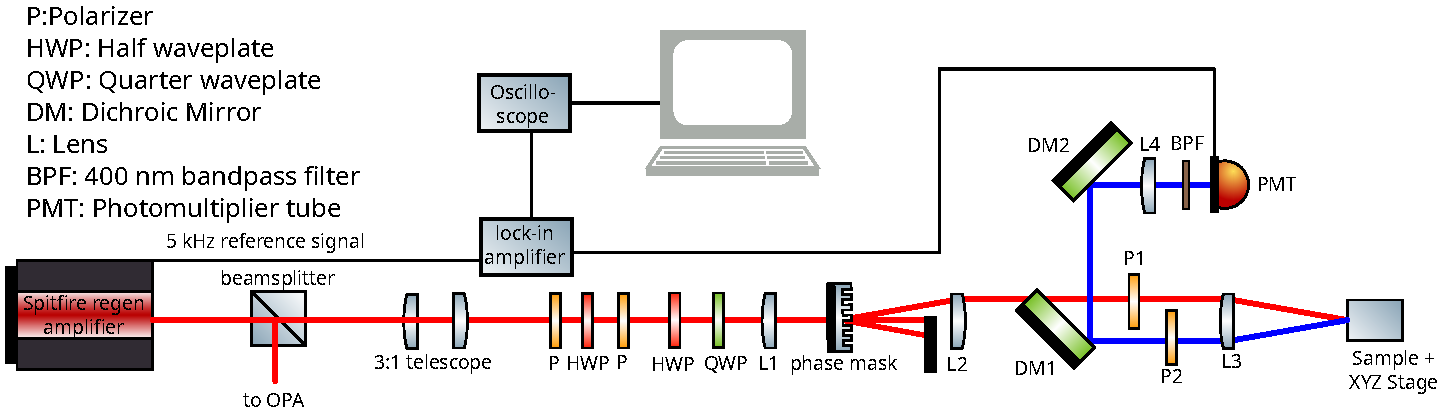
\includegraphics[width=\textwidth]{gfx/ch3/pdf/setup.pdf}
\caption[Schematic drawing of the SHG setup used in this research.]{\label{fig:setup}Schematic drawing of the \gls{shg} setup used in this research. After \citet{morey_automated_2024}.}
\end{figure}

With those considerations in mind, let me proceed to give a schematic description of our \gls{shg} setup (see \cref{fig:setup,fig:setup_real}).
Some of the choices we made may seem arbitrary right now, but I will go over them in detail in \cref{sec:beforeyoubuild}.
The starting point is our regenerative amplifier (Spectra-Physics Spitfire Sptf-100f-5k-xp), which produces $100$ \si{fs} $800$ \si{nm} pulses at a $5$ \si{kHz} repetition rate from an $86$ \si{MHz} seed laser (Spectra-Physics Tsunami 3941-M1S). 
$90\%$ of the beam is split off to power an \gls{opa}, and the remaining $10\%$ is used for the \gls{shg} probe beam.
After passing through an optical telescope, which creates a collimated beam of width $1-2$ \si{mm}, this beam is attenuated with a polarizer - half-wave plate - polarizer triplet, and then elliptically polarized with a quarter-wave plate and half-wave plate in series.
The ellipticity at this stage is set so the light is perfectly circularly polarized following transmission through a phase mask, as described below.

After passing through these polarization optics, the beam is focused with a lens onto the aforementioned phase mask, which acts as a transmissive diffraction grating and separates the beam into multiple different diffraction orders.
The $+1$ order diffraction comes off at an angle of roughly $7^\circ$, while the other orders are blocked with anodized aluminum foil. 
This (diverging) beam then propogates at $7^\circ$ to the optical axis before meeting a lens set at the appropriate distance so as to both collimate the beam and rectify the $7^\circ$ progation angle.
Then, the light passes through a dichroic mirror (which transmits $800$ \si{nm} and reflects $400$ \si{nm}), becomes linearly polarized by a wire-grid polarizer, and is then focused onto the sample at a $10^\circ$ angle of incidence by passing through the edge of a $1$ \si{in}-diameter $50$ \si{mm} achromatic focusing lens.
The interaction between the light and the sample causes \gls{shg} to be radiated in reflection at the same $10^\circ$ angle of incidence, so that the \gls{shg} beam passes through the opposite side of the $50$ \si{mm} lens before passing through a second, independent polarizer which is used to control the polarization of the measured light.

\begin{figure}
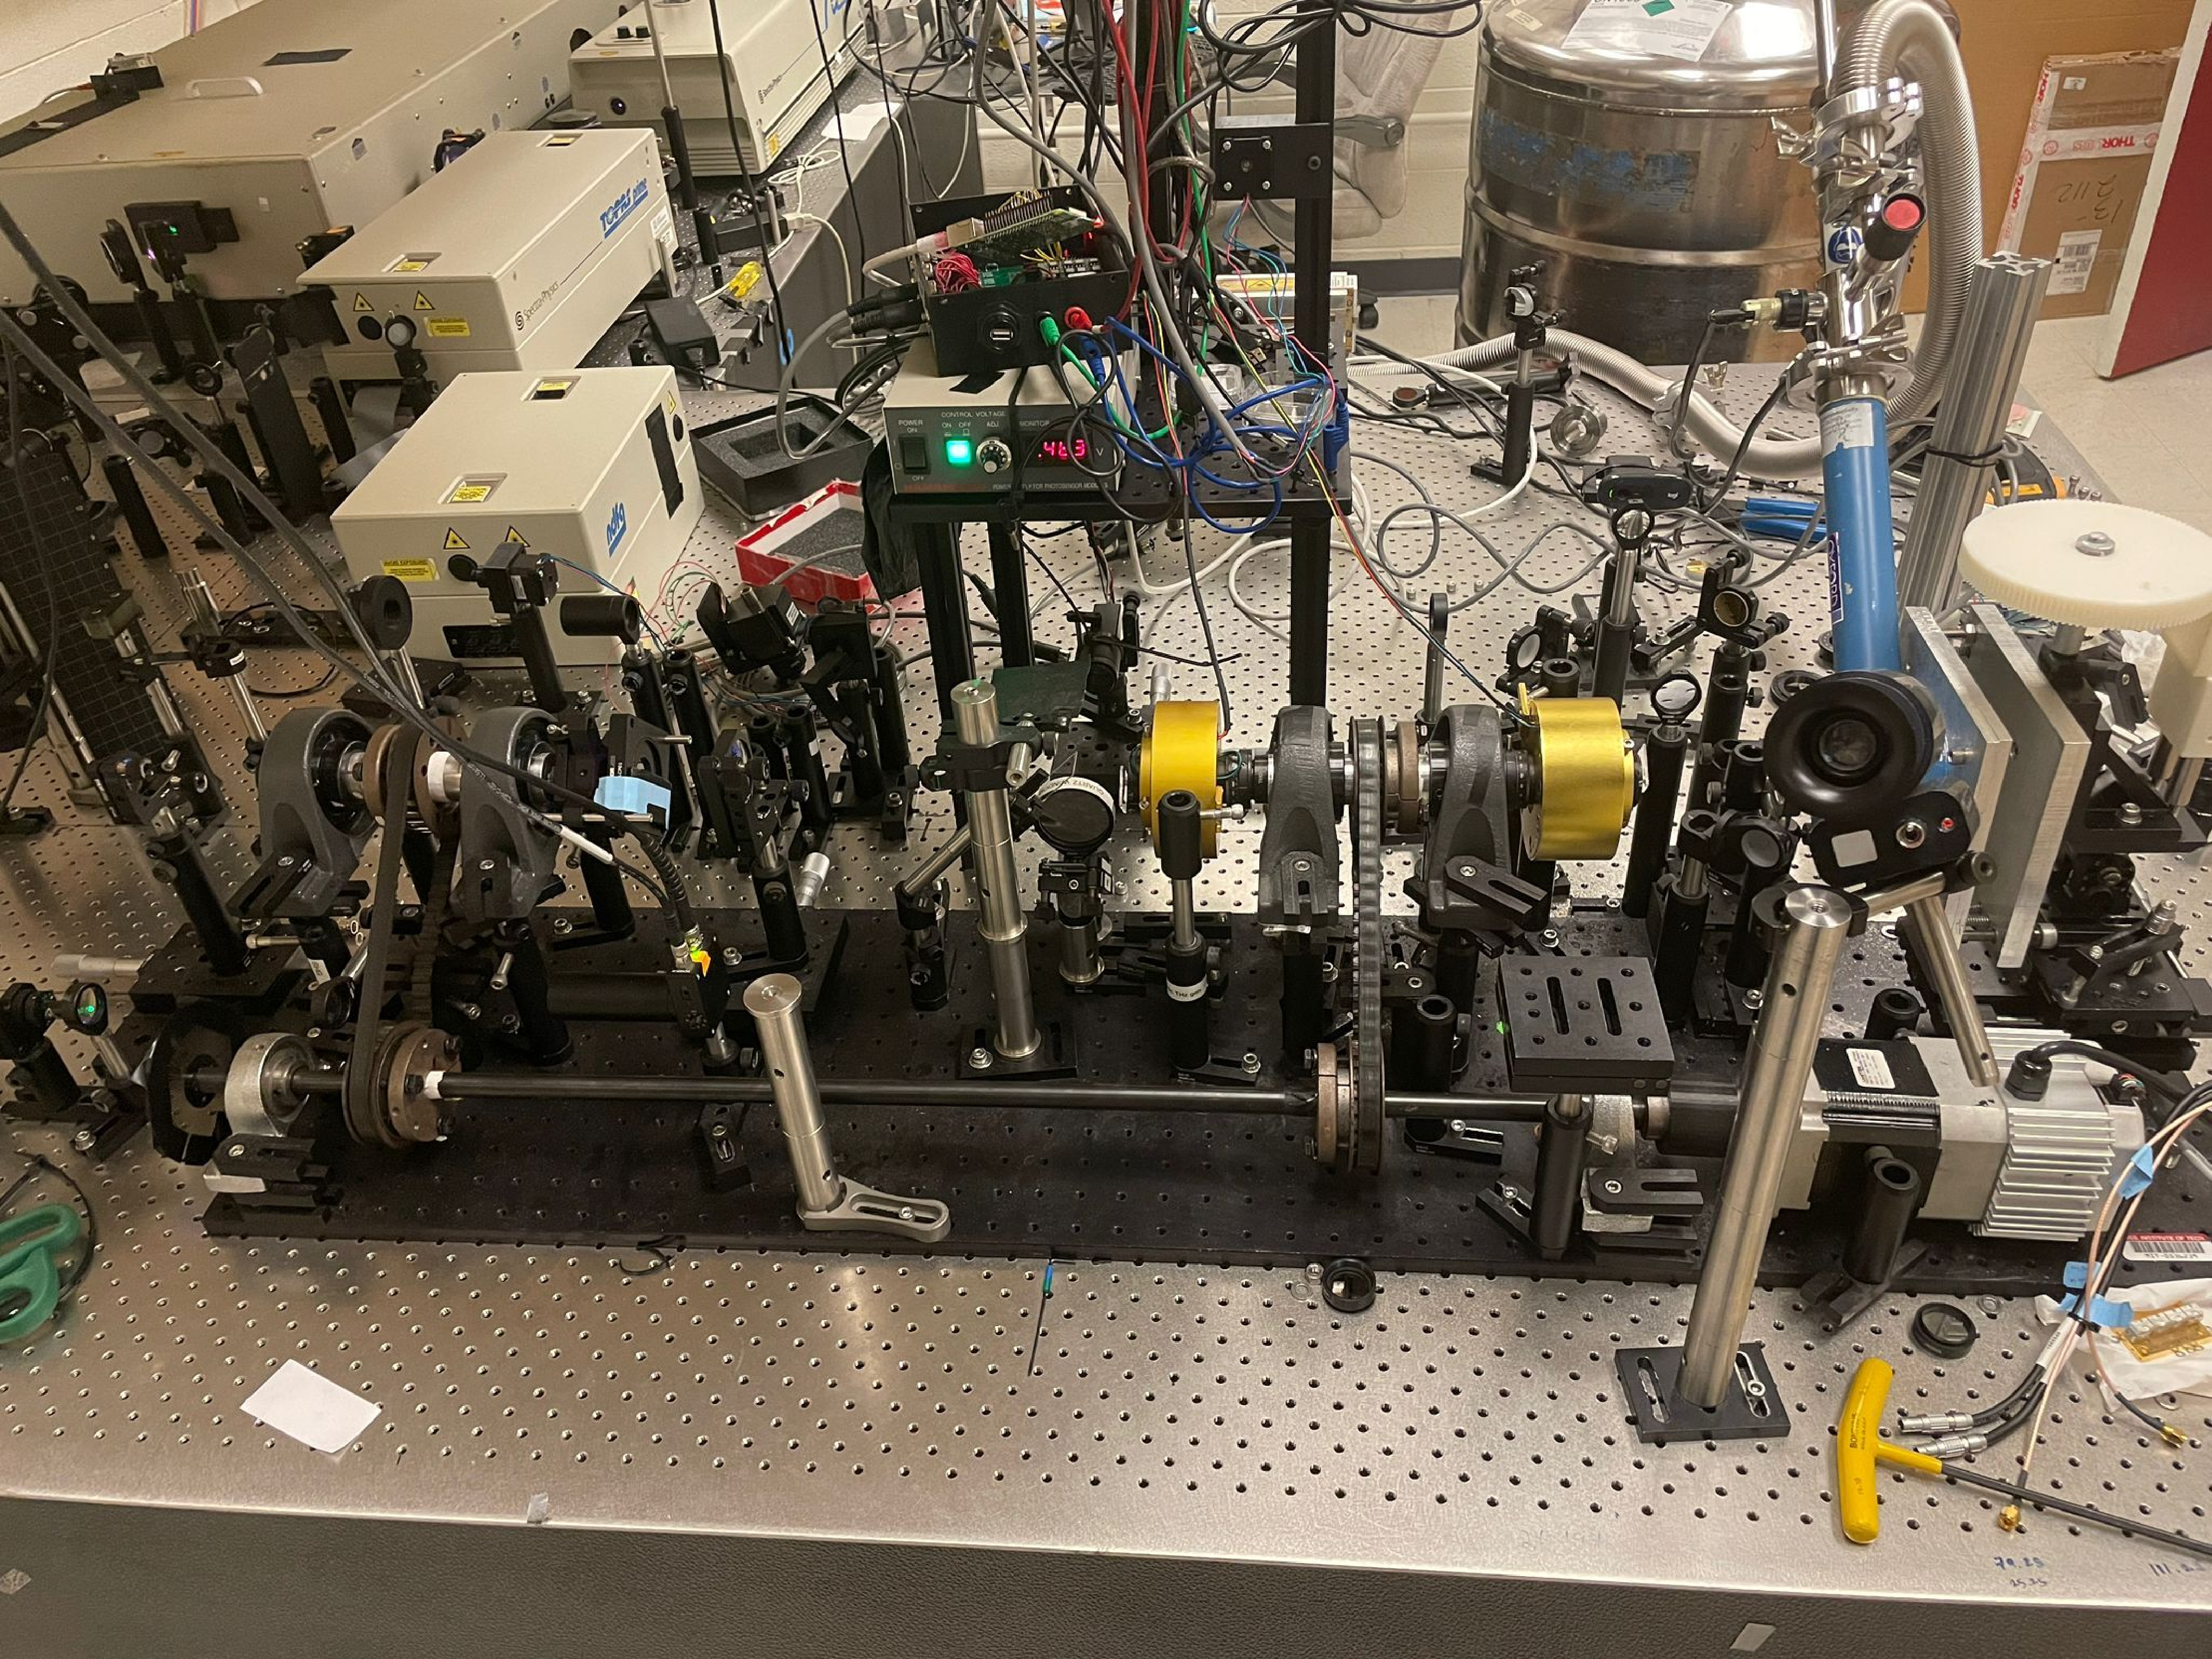
\includegraphics[width=\textwidth]{gfx/ch3/pdf/setup_real.pdf}
\caption[Photograph of the SHG setup.]{\label{fig:setup_real}Photograph of the \gls{shg} setup used in this research.
The sample lies in the blue cryostat on the right side of the image.
The phase mask is mounted in a black holder with blue masking tape on the left side, and the polarizers are mounted in the two gold-colored slip rings (described in \cref{ch:polrotators}).}
\end{figure}

Finally, the polarized output reflects off of two dichroic mirrors (oriented in such a way as to cancel the differing effect of the Fresnel equations on the reflectivity of S and P polarized light) and is focused through a $400$ \si{nm} bandpass filter onto a \gls{pmt} by a $400$ \si{mm} lens.
The current output of the \gls{pmt} is filtered by a lock-in amplifier (for static \gls{shg}, set to the $5$ \si{kHz} repetition rate of the laser) and read out on an oscilloscope.
The phase mask, incoming polarizer, and outgoing polarizer are mounted on rotating lens tubes which are connected via pulley to a common motor shaft driven at $\sim 5$ \si{Hz} by a brushless DC motor.
The motor thus continuously rotates the plane of incidence of the experiment, since the latter is entirely defined by the phase mask and the polarizers.
The rotation angle is tracked as a function of time by an optical rotary encoder, consisting of a laser pointer passed through a chopper wheel (with 100 slots) mounted at the end of the motor shaft and detected via photodiode.
The encoder signal and the lock-in signal are both sent to a homemade oscilloscope (an Arduino Uno microcontroller which separates the lock-in signal into different individual rotations by looking for peaks in the encoder signal), the output of which is sent to a computer for further data processing.

\section{Before you build}\label{sec:beforeyoubuild}

I list here a few essential aspects of \gls{shg} that should be considered before designing a new setup.

\subsection{Spot size}

One of the most important quantities in an \gls{shg} setup is the diameter of the probe spot.
Ideally, this diameter is as small as possible, so as to measure the smallest samples or domain sizes.
However, there is an important caveat: for constant fluence (i.e. supposing we are limited by the sample damage threshold), the \gls{shg} signal to noise ratio scales linearly in the area excited by the probe, and thus \gls{shg} microscopes have a difficult time measuring small \gls{shg} signals compared to traditional \gls{shg} setups with a larger excitation area.
To see this, let us say that our detector measures the number of photons per \gls{shg} pulse, which is proportional to the pulse energy $U_p(2\omega)$.
Assuming the input and output pulse intensity profiles have the shape of a square wave with width $\tau$ and height $I_p(\omega)$ and $I_p(2\omega)$, respectively, we have
\begin{equation}
U_p(2\omega) = A I_p(2\omega) \tau
\end{equation}
and
\begin{equation}
U_p(\omega) = A I_p(\omega) \tau
\end{equation}
where $A$ is the area of the beam at the sample surface.
The \gls{shg} intensity is proportional to the square of the input intensity
\begin{equation}
I_p(2\omega) \propto I_p^2(\omega)
\end{equation}
so that
\begin{equation}
U_p(2\omega) \propto \frac{U_p^2(\omega)}{A\tau}.
\end{equation}
Substituting for the fluence $f$
\begin{equation}
f(\omega) = \frac{U_p(\omega)}{A}
\end{equation}
we have
\begin{equation}
U_p(2\omega) \propto \frac{f^2(\omega)A}{\tau}
\end{equation}
i.e., if we hold the fluence constant at the sample damage threshold, the number of photons in the generated \gls{shg} pulse is proportional to the excitation area and inverse to the pulse width.
The signal to noise ratio is then given by
\begin{equation}
\mathrm{SNR} \propto \frac{U_p(2\omega)}{\sqrt{r}}
\end{equation}
where $r$ is the system repetition rate.

\subsection{Oblique vs. normal incidence}\label{sec:obliquevsnormal}

While all of the results presented in this thesis utilized the setup in \cref{fig:setup}, where the incident beam makes a small angle with respect to the sample normal, plenty of groups use a different approach where that angle is set to $0^\circ$.
This has the obvious disadvantage of not specifying all of the tensor elements, since any element $\chi_{ijk}$ with $i, j, k = z$ is not accessible in this geometry.
However, in some cases this can actually be something of an advantage.
For example, sometimes unwanted \gls{shg} contributions (see \cref{sec:manyshgterms}) may be avoided in the normal incidence geometry, assuming the \gls{na} of the focusing optic is small enough that longitudinal components of the electric field are nearly zero.
Furthermore, in some materials the order parameter only couples to one or two elements of $\chi_{ijk}$; if none of these elements have a $z$ index, it is needless to complicate the analysis with oblique incidence.

In my experience, oblique incidence seems to be useful in two broad cases.
For one thing, some order parameters only show up in the $z$ components of $\chi_{ijk}$ (this is the case in \tastwo, see \cref{ch:tastwo}), in which case one obviously needs a nonzero angle of incidence to access these components.
A more subtle point is that, even if in practice all of the phenomenology of a particular sample only shows up in the $x$ and $y$ indices of $\chi_{ijk}$, still one must measure the full tensor to \emph{rule out} unseen phenomenology in the other indices.
Both the \ce{CaMn2Bi2} (\cref{ch:cmb}) and \ce{CuBr2} (\cref{ch:cubr2}) works presented in this thesis are examples of exactly this point, where the main scientific arguments involve either comparing \gls{shg} patterns in two domains or comparing oscillation amplitudes in different polarization channels.
Clearly one needs to know all of the tensor elements to make those arguments exact.

\subsection{Choice of detector}

Our setup is somewhat unique in using a \gls{pmt} for data collection rather than an \gls{emccd}, which is the slightly more traditional method.
Frankly, this decision was not based on the detection efficiency, but rather the fact that \glspl{pmt} typically cost about two orders of magnitude less than \glspl{emccd}.
However, the setup construction with a \gls{pmt} is slightly different than with an \gls{emccd}, so you should probably decide which you want to use before you start building your setup.
With an \gls{emccd}, the beam is sent into the device without focusing (L4 in \cref{fig:setup}) so that the beam traces a circle on the sensor as a function of time\cite{harter_high-speed_2015}.
The rotational anisotropy signal is read off by performing a radial integration of the camera image (after masking the part of the image which is outside from the circle traced by the beam).
In this way, the rotation angle of the motor is correlated with the \gls{shg} signal via the azimuthal degree of freedom on the camera image.
In contrast, with a \gls{pmt} the \gls{shg} signal is read out as a function of time on an oscilloscope (see \cref{sec:setupdescription}), and must be correlated with the rotation angle of the motor by some other method.
We use an optical chopper wheel attached to the motor shaft; a beam from a laser pointer is directed through the chopper wheel and onto a photodiode, which produces a square wave signal that is used to trigger the oscilloscope.
One must also be careful that the \gls{pmt} is aligned as close to normal as possible to the axis defined by DM2 and L4 in \cref{fig:setup}, as the \gls{pmt} output is actually quite sensitive to the angle of incidence of the input radiation.

As for the detection efficiency of the two devies, an \gls{emccd} is basically an \emph{array} of \glspl{pmt}---thus, there is no fundamental difference in the detection efficiences of the two methods, although having never used an \gls{emccd} I cannot speak to any specific considerations that might favor one over the other.

\section{tr-SHG: methodology}

\subsubsection{Polarization control}

The main limitation for doing \gls{trshg} is simply that the experiment becomes longer.
Each measurement of $\chi_{ijk}$ requires averaging four different polarization channels (\PP, \PS, \SP, and \SS), which, depending on the signal to noise ratio, can take as long as $2-3$ minutes each.
In a time-resolved experiment, that procedure must be repeated at least once for each time delay; in fact, it us often useful to sweep the delay stage multiple times to reduce the extent to which systematic drifts in in the laser power, alignment, etc. affect the time trace.
Not only is this time-consuming (typically taking $\sim 12$ \si{hours} to get a good dataset), but it also requires four rotations of the polarizers at each delay, which is simply not feasible if the polarizers are to be rotated manually.
Unfortunately, automated polarizer rotation is difficult in the \gls{rashg} experimental geometry because the polarizers must be rotated relative to a lens tube which is \emph{itself} rotating at $5$ \si{Hz}.
The traditional method of rotating polarizers via stepper motor is thus not possible, unless one finds a method to transmit power between the stationary laboratory frame and the rotating frame that the polarizer lives in.
Myself and Karna Morey designed such a method using an electronic device known as a hollow-bore electric slip ring, which uses ring-shaped conductive pads in combination with low-friction metallic brushes to conduct electricity between two rotating objects.
In my opinion, such a design is essential to doing \gls{trshg} unless one is satisfied with only measuring a single polarization channel; thus, I have dedicated the entirety of \cref{ch:polrotators} to our solution, which in my opinion represents the largest contribution we made to \gls{shg} methodology during this thesis.

\subsubsection{The pump beam path}

Having discussed the modifications needed for \gls{trshg} on the probe arm, let us now describe the pump beam path.
$100$ \si{fs} pulses from the regenerative amplifier (Spectra-Physics Spitfire Sptf-100f-5k-xp) are split by $90:10$ beamsplitter (with the $10\%$ becoming the probe beam, see \cref{sec:setupdescription}) and are used as input to an \gls{opa} (Light Conversion TP8F1N3) which produces light of variable wavelength between $1100$ and $2080$ \si{nm}.
The output of the \gls{opa} is directed through a wire-grid polarizer (to pick out the signal or idler, as needed) to an optical delay line (Newport DL125 with SMC100 motion controller) and a second polarizer to vary the beam power.
The beam then passes through a \gls{nir} longpass filter to remove unwanted visible wavelengths that are output by the \gls{opa}.
A $400$ \si{nm} lens focuses the beam past two mirrors (one mounted with epoxy onto the focusing lens L3 of \cref{fig:setup}\footnote{Remember that the probe beam is arriving at oblique incidence and thus passes through the edge, rather than the center, of L3.}) and finally onto the sample.
The diameter of the pump beam at the focus is set by moving the lens position along the beampath and monitoring the beam shape with a CCD camera.
The pointing of the beam is aligned so that the light reflected off the sample is perfectly backscattered.
Pump scatter is avoided by mounting a small black circular disk in the center of L3, and by subtracting ``dark'' scans without the probe beam from the final dataset.

An optical chopper wheel is placed somewhere in the pump beam path which blocks every other pulse from the \gls{opa}, so that the effective repetition rate of the pump pulsetrain is $2.5$ \si{kHz}.
The output of the \gls{pmt} (see \cref{fig:setup}) is sent to a lock-in amplifier synced to this frequency, so that the output of the lock-in is proportional to
\begin{equation}
I^\mathrm{SHG}_{\mathrm{Pump}+\mathrm{Probe}} - I^\mathrm{SHG}_\mathrm{Probe}
\end{equation}
i.e. the output of the lock-in is the pump-induced change in the measured \gls{shg} intensity.

Finally, the pump-probe time delay is varied, and for each delay the rotational anisotropy in the \gls{shg} intensity is measured in each of the four polarization channels.
Alternatively, the motor rotation may be parked at a fixed angle and the \gls{shg} intensity at this angle measured as a function of delay time.

\section{Data analysis}\label{sec:dataanalysis}

Finally, we discuss the analysis of \gls{shg} data, first in the static limit and then in the context of \gls{trshg}.

\subsection{Static RA-SHG patterns}\label{sec:staticanalysis}

The typical static \gls{rashg} dataset consists of a set of points $\{(\phi_n, I^p_n)\}$, $n \in \{0, 1, \ldots N-1\}$ and standard errors $\{\sigma^p_n\}$ for each of the four independent polarization channels
\[
p\in\{\mathPP, \mathPS, \mathSP, \mathSS\}.
\]
By \cref{eq:shgsimple}, each of these patterns may be modeled by an equation\footnote{I will focus on electric dipole \gls{shg} for now, although note that the equations for electric quadrupole and magnetic dipole \gls{shg} (\cref{eq:mshort,eq:qshort}) are different---by \cref{eq:sourceterm}, both involve a factor of the incident wavevector $\bm{k}$, and the magnetic dipole term has a cross product.}
\begin{equation}\label{eq:fundamentalmodel}
I^p(\phi) \propto |\hat{e}_i^{p,\mathrm{out}}(\phi)\chi_{ijk}\hat{e}_j^{p,\mathrm{in}}(\phi)\hat{e}_k^{p,\mathrm{in}}(\phi)|^2,
\end{equation}
where $\hat{\bm{e}}$ is a unit vector in the direction of the corresponding electric field.
These unit vectors are given as a function of $\phi$ and the angle of incidence $\theta$ in \cref{tab:polarizations}.

\begin{landscape}
\begin{table}
\renewcommand{\arraystretch}{1.1}
\caption[Vector definition of polarization channels.]{\label{tab:polarizations}Vector definition of polarization channels. $\theta$ is the angle of incidence and $\phi$ is the angle of the plane of incidence with respect to the $\hat{x}$ axis.}
\begin{tabular}{|c c|c c c|c c c|}
\hline
\multirow{2}{*}{Input} & \multirow{2}{*}{Output} & \multicolumn{3}{|c|}{$\hat{\bm{e}}^\mathrm{in}(\phi)$} & \multicolumn{3}{|c|}{$\hat{\bm{e}}^\mathrm{out}(\phi)$}\\
& & $\hat{e}^\mathrm{in}_x(\phi)$ & $\hat{e}^\mathrm{in}_y(\phi)$ & $\hat{e}^\mathrm{in}_z(\phi)$ & $\hat{e}^\mathrm{out}_x(\phi)$ & $\hat{e}^\mathrm{out}_y(\phi)$ & $\hat{e}^\mathrm{out}_z(\phi)$\\
\hline
P & P & $\cos\phi\cos\theta$ & $\sin\phi\cos\theta$ & $-\sin\theta$ & $-\cos\phi\cos\theta$ & $-\sin\phi\cos\theta$ & $-\sin\theta$\\
P & S & $\cos\phi\cos\theta$ & $\sin\phi\cos\theta$ & $-\sin\theta$ & $-\sin\phi$ & $\cos\phi$ & $0$\\
S & P & $-\sin\phi$ & $\cos\phi$ & $0$ & $-\cos\phi\cos\theta$ & $-\sin\phi\cos\theta$ & $-\sin\theta$\\
S & S & $-\sin\phi$ & $\cos\phi$ & $0$ & $-\sin\phi$ & $\cos\phi$ & $0$\\
\hline
\end{tabular}
\end{table}
\end{landscape}

Let us assume that we know the point group $P_G$ of our material.
Then, the first step is to constrain the values of $\chi_{ijk}$ using the arguments of \cref{sec:neumann}.
One can do this manually by solving the system of equations defined by \cref{eq:nmindex}, or one can simply look up the answer in one of a number of tables (e.g. \citet{boyd})\footnote{Be aware that these tensors are given in just one of many choices of coordinates; a rotation of $\chi_{ijk}$ may be needed to agree with the orientation of the crystal in the experiment.}; in the end we are left with a tensor $\chi_{ijk}^{P_G}$ with $M$ independent elements $\{\chi_i, i\in 0, 1, \ldots, M-1\}$.

The goal is to simultaneously fit the four patterns $\{(\phi_n, I^p_n\}$ to \cref{eq:fundamentalmodel} using the $\chi_i$'s.
Our objective function is thus
\begin{equation}
f(\{\chi_i\}) = \sum_{\substack{p\in \{\mathPP, \mathPS,\\ \mathSP, \mathSS\}}}\sum_{n=0}^{N-1}\left(\frac{I^p(\phi_n) - I^p_n}{\sigma^p_n}\right)^2
\end{equation}
with $I^p(\phi)$ defined in \cref{eq:fundamentalmodel}.
Unfortunately, such a function is quite difficult to minimize.
The reason is that $I^p(\phi)$ is ultimately a sum of products of trigonometric functions of $\phi$ (due to \cref{tab:polarizations}) which can be difficult for typical minimization algorithms.
An alternative is to cast the problem in terms of the \glspl{ft}
\begin{equation}\label{eq:ftmodel}
\ft{I}^p(k) \equiv \frac{1}{2\pi}\int_0^{2\pi}I^p(\phi)e^{-i k\phi} \, d\phi
\end{equation}
of $I^p(\phi)$ and the \glspl{dftr}
\begin{equation}
\{(k, \ft{I}^p_k)\},
\end{equation}
of $\{(\phi_n, I^p_n)\}$, where\footnote{I am assuming the $\phi_n$'s are equally spaced.}
\begin{equation}
\ft{I}^p_k \equiv \frac{1}{N}\sum_{n=0}^{N-1}I^p_n e^{-ik\phi_n}.
\end{equation}
Since the \gls{dftr} is unitary, the uncertainties $\ft{\sigma}^p_k$ are simply the \gls{dftr} of the $\sigma^p_n$'s.
Thus, our new objective function is
\begin{equation}\label{eq:objectivefunction}
f(\{\chi_i\}) = \sum_{\substack{p\in \{\mathPP, \mathPS,\\ \mathSP, \mathSS\}}}\sum_{k=0}^{N-1}\left(\frac{\ft{I}^p(k) - \ft{I}^p_k}{\ft{\sigma}^p_k}\right)^2.
\end{equation}
This is a much easier function to minimize for two reasons: one, the function is now just a quadratic function of the $\{\chi_i\}$'s, and two, since there are only six factors of trigonometric functions of $\phi$ in $I^p(\phi)$, $\ft{I}^p(k) = 0$ for $k \notin \{-6, -5, \ldots, 6\}$\footnote{This is the case for electric dipole \gls{shg}; for electric quadrupole and magnetic dipole, we can have as much as $k = \pm 8$.} (the other terms in \cref{eq:objectivefunction} just contribute an overall constant to $f$).

What is left then is just the choice of minimization algorithm.
Unfortunately, simple gradient descent algorithms are not ideal here unless you have a really good initial guess, since \cref{eq:ftmodel} is still quadratic in the fitting parameters and the global minimum is often surrounded by many local minima which can easily cause these algorithms to become trapped.
Global minimization routines are thus optimal; I have used the simulated annealing algorithm of \citet{xiang_generalized_1997} with success, as well as the related ``basinhopping'' algorithm of \citet{wales_global_1997}, both of which are implemented in \texttt{scipy.optimize}\citep{scipy}.
Ultimately, though, it is up to the experimenter to ensure they have found the true global minimum of \cref{eq:objectivefunction}.

As part of this thesis, I wrote a software package in Python called ShgPy which uses \texttt{sympy}\citep{sympy} to compute the \gls{ft} model \cref{eq:ftmodel} and \texttt{scipy.optimize}\citep{scipy} to fit this model to the data via \cref{eq:objectivefunction}.
Installation instructions and a comprehensive documentation may be found at the project home page \url{https://bfichera.github.io/shgpy/}.

\subsection{Modeling $\chi_{ijk}$: the simplified bond hyperpolarizability model}

Sometimes the symmetry-constrained $\chi_{ijk}$ of \cref{sec:staticanalysis} is difficult to analyze (perhaps it has too many fitting parameters), in which case it might be prudent try and justify an even more tightly constrained $\chi_{ijk}$ via some a microscopic model.
We have already seen two such models via \cref{eq:bigshg,eq:sashg}, but the former is typically not tractable and the latter may only be valid in the presence of a spontaneous symmetry-breaking phase transition with a well-defined order parameter.
One alternative is to model the microscopic charge degrees of freedom classically---suppose most of the motion of charges in our solid occurs in the bonds between atoms, and that that motion is constrained to occur along the bond direction only.
Then, the solid can be modeled as an ensemble of oscillating dipoles (one for each bond in the unit cell) with corresponding hyperpolarizabilities $\{\alpha_n\}$.
Symmetry may dictate how many independent $\alpha_n$'s there are in the unit cell, but otherwise these are considered unknown and to be fit to the data.
The electric dipole \gls{shg} response of such an ensemble was analyzed by \citet{powell_simplified_2002}, and the electric quadrupole response was later considered by \citet{bauer_bulk_2017}; the answer in both cases is quite simple:
\begin{align}
\chi^{eee}_{ijk} &= \sum_n \alpha_n b^n_i b^n_j b^n_k\label{eq:esbhm}\\
\chi^{qee}_{ijkl} &= \sum_n \gamma_n b^n_i b^n_j b^n_k b^n_l\label{eq:qsbhm}
\end{align}
where $\bm{b}^n$ is a unit vector in the direction of bond $n$ and the $\alpha_n$'s and $\gamma_n$'s are the unknown parameters of the dipole and quadrupole models, respectively.

When valid, this \gls{sbhm} is powerful for two reasons: for one, \cref{eq:esbhm,eq:qsbhm} typically have fewer unknown parameters than the naive, symmetry-constrained tensor $\chi_{ijk}^{P_G}$ of \cref{sec:staticanalysis}, and two, there is a direct connection between the unknown parameters $\alpha_n$ and $\gamma_n$ and the microscopic degrees of freedom.
One can thus draw conclusions \emph{about} the microscopic degrees of freedom by fitting the \gls{shg} patterns to \cref{eq:esbhm,eq:qsbhm} (see, e.g., \citet{ron_dimensional_2019}).
Of course, one must be careful that the assumptions of this model---that the charges are localized to the bonds, and that the only relevant motion is along the bond direction---are actually correct before proceeding with this sort of analysis.

Myself and Karna Morey built a comprehensive interface to the \gls{sbhm} in Python using \texttt{pymatgen}\citep{ong_python_2013}, which takes an arbitrary \gls{cif} and calculates the relevant susceptibility tensors via \cref{eq:esbhm,eq:qsbhm}.
The change to the susceptibility tensor induced by an elastic distortion mode ($\chi_{ijk}(q)$, where $q$ is the mode amplitude) can be computed via integration with \texttt{ISODISTORT}\citep{isodistort, campbell_isodisplace_2006}.
See the package documentation (\url{https://github.com/morey18k/sbhm.git}) for examples and further information.

\subsection{Fitting time traces in tr-SHG}

As the final section of this chapter, let me remark on a few aspects of fitting time-domain signals that are not necessarily specific to \gls{shg}, but are nevertheless essential for \gls{trshg} analysis.

Typically, in \gls{trshg} we plot the pump-induced change in the \gls{shg} intensity at a single angle $\phi_0$ as a function of the delay time $t$; more complicated analysis of the tensor elements themselves is possible but often unnecessary.
This intensity change $\Delta I_{2\omega}(t, \phi_0)$ is related to $P(2\omega)$ via
\begin{align}
\Delta I_{2\omega}(t, \phi_0) &= I_{2\omega}^{\mathrm{Pump}+\mathrm{Probe}}(t, \phi_0)-I_{2\omega}^\mathrm{probe}(0, \phi_0)\\
&\propto |P_{2\omega}(0, \phi_0)+\delta P_{2\omega}(t, \phi_0)|^2 - |P_{2\omega}(0, \phi_0)|^2\\
&\propto 2P_{2\omega}(0, \phi_0)\delta P_{2\omega}(t, \phi_0) + |\delta P_{2\omega}(t, \phi_0)|^2
\end{align}
where we have used that the signal is presumably independent of time if there is no pump pulse.
When $|\delta P_{2\omega}(t, \phi_0)| \ll |P_{2\omega}(0, \phi_0)|$, this reduces to
\begin{equation}
\Delta I_{2\omega}(t, \phi_0) \propto P_{2\omega}(0, \phi_0)\delta P_{2\omega}(t, \phi_0).
\end{equation}

The basic problem is then that we have a dataset 
\begin{equation}
\{t_n, I_n\}, n\in \{0, 1, \ldots, N-1\}
\end{equation}
with uncertainties $\sigma_n$ which we wish to fit to some model, typically consisting of some (e.g. polynomial) background
\begin{equation}
b(t, \{b_k\}), k\in\{0, 1, \ldots, K-1\}
\end{equation}
plus $1$ to $M$ damped harmonic oscillators
\begin{equation}
I(t, \params) = \begin{cases}
0 & t<0\\
b(t, \{b_k\})+\sum_{m=1}^M A_m e^{-t/\tau_m} \cos (2\pi f_m t + \psi_m) & t>0
\end{cases},
\end{equation}
where $\params$ refers to the set of unknown parameters $\{b_k\}$, $\{A_m\}$, $\{\tau_m\}$, $\{f_m\}$, and $\{\psi_m\}$.
We wish to determine the model coefficients $\params$ by minimizing the objective function
\begin{equation}\label{eq:trobjectivefunction}
f(\params) = \sum_{n=0}^{N-1}\left(\frac{I(t_n, \params)-I_n}{\sigma_n}\right)^2.
\end{equation}

Various algorithms exist to find the minimum $\params_0$ of $f$; the \gls{lm} algorithm \citep{levenberg_method_1944,marquardt_algorithm_1963} is known to have trouble with exponential functions, so it is recommended to do a Nelder-Mead search \citep{nelder_simplex_1965} first and then use \gls{lm} to refine the solution.
These methods also report the uncertainties $\{\sigma_i\}$ on each fitting parameter, basically by computing the curvature of the function $f$ near $\params_0$ (which depends, among other things, on the data uncertainty $\{\sigma_n\}$).
Importantly, however, these uncertainties are only valid when $f$ is a linear function of the model parameters near the minimum!\footnote{Here, ``near'' means ``in a neighborhood of size $\sigma_i$.}
This is a point which is completely overlooked in the ultrafast condensed matter literature, even though there is really no reason that \cref{eq:trobjectivefunction} should satisfy this criterion for typical uncertainty levels in pump-probe experiments.

The correct approach in this case is to note that the data set $D_0 \equiv \{t_n, I_n\}$ is just one of many possible datasets $D_0, D_1, D_2, \ldots$ that we \emph{could} have measured during our experiment.\footnote{The following discussion closely follows that of \textit{Numerical Recipes}, chapter 15\citep{numericalrecipes}.}
If we could run the minimization procedure described above for each of these hypothetical datasets, we would end up with a whole distribution of model coefficients $\params_0, \params_1, \params_2, \ldots$ from which our measurement $\params_0$ was just a single draw.
The spread of this distribution (or, more precisely, the spread of the distribution $\params-\params_\mathrm{true}$) reflects exactly the quantitative uncertainty in our measurement of $\params$ that we would like to report.

Our goal, then, is to approximate this distribution by some method.
One approach (which works when we have many observations $\{t, I\}$ with the same $t$) is called the nonparametric bootstrap\citep{cressie}.
For each time $t_n$, let us say that we have a set of measured intensities $\{I^n_m\}$, with $m\in \{1, 2, \ldots, M_n\}$.
Then, we generate new hypothetical datasets $\mathscr{D}_1, \mathscr{D}_2, \ldots$ by (for each $t_n$) drawing $M_n$ items \emph{with replacement} from the $\{I^n_m\}$'s.
The fact that this new distribution of datasets is a faithful representation of the true distribution $\{D_0, D_1, D_2, \ldots\}$ is not obvious, but theoretical work by many authors (see \citet{wackernagel} for a review) has established that it is nevertheless true.

If we are confident that our model $I(t, \params)$ is, in fact, the true model (at least for some set of coefficients $\params_\mathrm{true}$), then rather than using the dataset $D_0$ to generate our hypothetical datasets, we can instead choose to use the model \emph{itself}.
The idea is to take our estimate $I(t, \params_0)$ and generate new datasets $\{\mathscr{D}_m\}$ essentially by adding noise:
\begin{equation}\label{eq:parametricbootstrap}
\mathscr{D}_m = \{(t_n, I(t_n, \params_0)+N_n), n\in \{0, 1, \ldots, N-1\}\},
\end{equation}
for some random variable $N_n$ which we put in by hand.
This is called the parametric bootstrap, referring to the fact that we are estimating our true distribution $\{D_0, D_1, D_2, \ldots\}$ via the parameters $\params_0$\citep{dekking}.
In order for the distribution of $\mathscr{D}_m$'s to faithfully represent the true distribution $\{D_0, D_1, D_2, \ldots\}$, obviously $N_n$ needs to reflect the actual noise distribution of the experiment.
Thankfully, in pump-probe experiments, we usually know this distribution---as long as we have enough points $(t_n, I_n)$ with $t_n<0$, we can estimate $N_n$ with a normal distribution centered about $0$ with variance $\left<(I_n)^2\right>_{<0} - \left<I_n\right>_{<0}^2$, where $\left<\cdot\right>_{<0}$ means ``average over points with $t_n<0$.''

Once we have the hypothetical datasets $\{\mathscr{D}_m\}$ (regardless of how we generated them), we proceed by estimating a $\params_m$ for each one using \cref{eq:trobjectivefunction}, and then plotting the distribution $\{\params_m - \params_0\}$; the spread of this distribution tells us the uncertainties $\sigma_i$ in each of our model coefficients.
The important part is that these uncertainties are much more reflective of the true uncertainty in our measurement of $\params$ than the curvature of \cref{eq:trobjectivefunction} near $\params_0$, which we have argued is strictly incorrect in many cases.
